\chapter{The R1 Sweep: Corrected-Optics Blur-Only Optimum}
\label{ch:r1sweep}

This chapter presents the full corrected-optics blur-minimization sweep --- this
project's headline result --- across the complete $15\times8$ grid, with no brightness
or acuity constraint applied (Chapters~\ref{ch:stage3a} and~\ref{ch:acuity_models} add
those separately). \textbf{Every result in this chapter is computed and shown for all
four encircled-energy percentiles the pipeline reports at every point} ---
$r_{EE}(50\%)$, $r_{EE}(70\%)$, $r_{EE}(80\%)$, and $r_{EE}(90\%)$
(Section~\ref{sec:effective-radius}) --- not for $r_{EE}(50\%)$ alone.

\section{All four percentiles, full grid}
\label{sec:r1-all-percentiles}

Figure~\ref{fig:r1-lines-all} shows blur vs.\ aperture, one panel per percentile, one
line per myopia level within each panel. Every curve at every percentile is
U-shaped: diffraction dominates at small apertures (blur decreases as the aperture
grows), while defocus dominates at large apertures (blur increases again as more of
the eye's uncorrected myopic power is exposed) --- the aperture-size trade-off this
whole report is built around, and a shape that holds regardless of which percentile is
used. Figure~\ref{fig:r1-heatmap-all} shows the identical data as four
aperture$\times$$M$ heatmaps.

\begin{figure}[htbp]
\centering
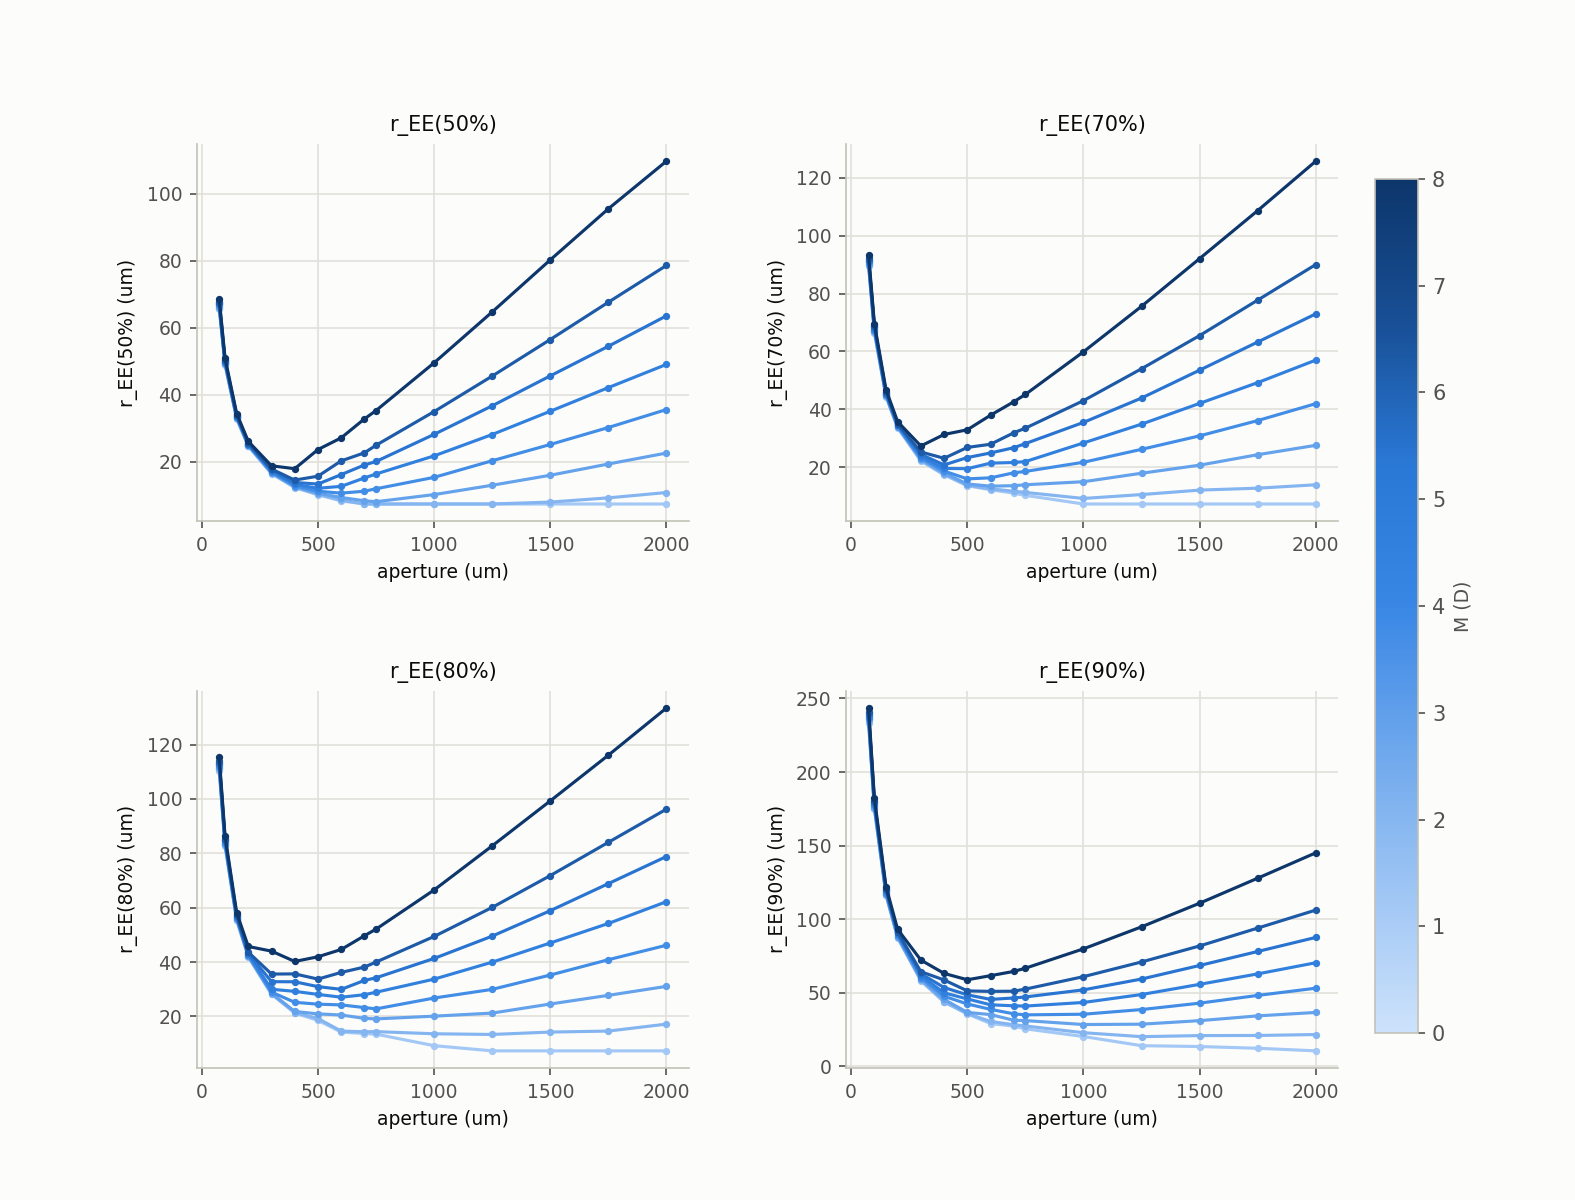
\includegraphics[width=\textwidth]{figures/fig_r1_lines_all_percentiles.png}
\caption{Corrected-optics blur vs.\ aperture, all four percentiles, one line per myopia level $M$ within each panel (sequential blue colormap, darker = higher $M$).}
\label{fig:r1-lines-all}
\end{figure}

\begin{figure}[htbp]
\centering
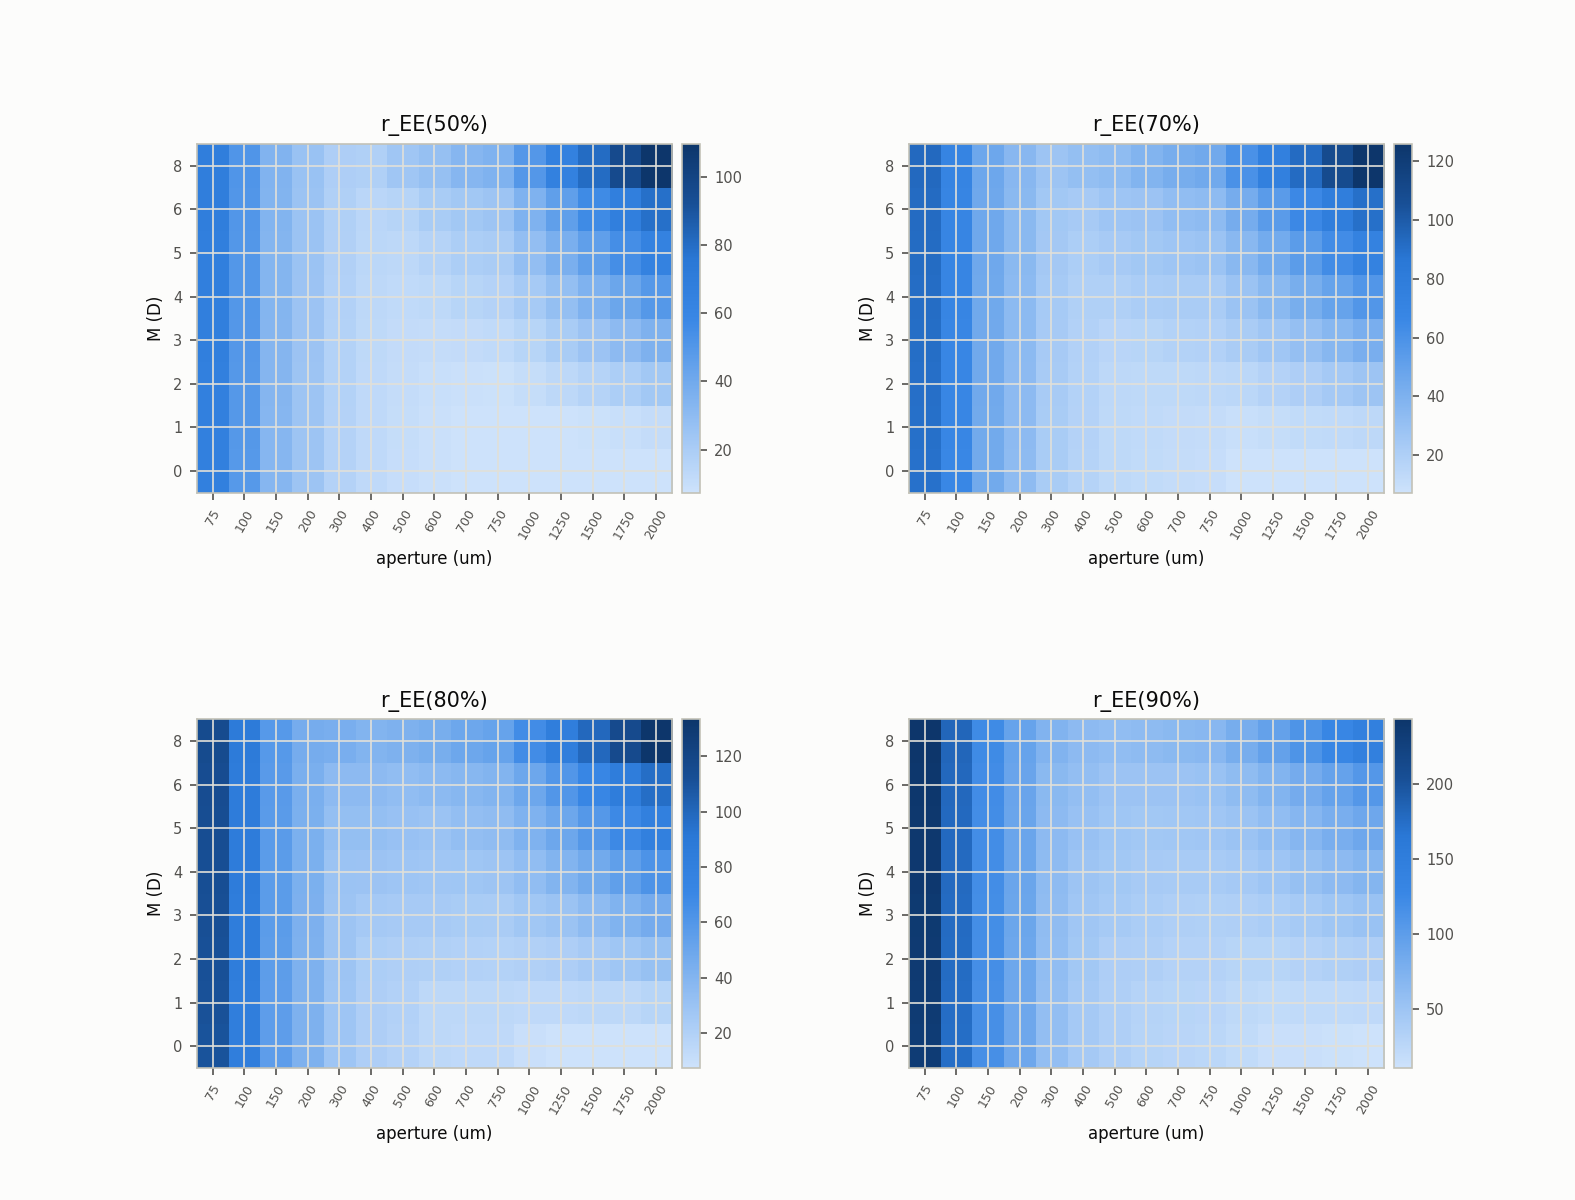
\includegraphics[width=\textwidth]{figures/fig_r1_heatmap_all_percentiles.png}
\caption{Corrected-optics blur (\textmu m) across the full aperture $\times$ myopia grid, all four percentiles.}
\label{fig:r1-heatmap-all}
\end{figure}

{\small
\begin{longtable}{rrrrr}
\caption{Unconstrained blur-only optimal aperture (um), all four percentiles, per myopia level.}\label{tab:r1-all-percentiles}\\
\toprule
M (D) & r\_EE(50\%) & r\_EE(70\%) & r\_EE(80\%) & r\_EE(90\%) \\
\midrule
\endfirsthead
\multicolumn{5}{c}{\tablename\ \thetable\ -- continued}\\
\toprule
M (D) & r\_EE(50\%) & r\_EE(70\%) & r\_EE(80\%) & r\_EE(90\%) \\
\midrule
\endhead
\bottomrule
\endfoot
0 & 700 & 1000 & 1250 & 2000 \\
1 & 700 & 1000 & 1250 & 1250 \\
2 & 750 & 600 & 750 & 1000 \\
3 & 600 & 500 & 750 & 750 \\
4 & 500 & 500 & 600 & 750 \\
5 & 500 & 400 & 600 & 600 \\
6 & 400 & 400 & 500 & 600 \\
8 & 400 & 300 & 400 & 500 \\
\end{longtable}
}

The optimal aperture is not the same number across percentiles, and the choice
matters: at $M=8\,$D it ranges from $300\um$ ($r_{EE}(70\%)$) to $500\um$
($r_{EE}(90\%)$) --- a $67\%$ spread from changing only which fraction of encircled
energy is minimized, with no other assumption changed at all.
\textbf{Important caveat, carried forward from this exact table}: the $M=0$ and
$M=1$ columns for $r_{EE}(70\%)$ and $r_{EE}(80\%)$ are not genuine unique minima ---
Chapter~\ref{ch:percentile} identifies and quantifies a grid-resolution saturation
artifact at those two myopia levels specifically, and should be read before treating
those two rows at face value. $M\ge2$ rows are unaffected and trustworthy.

\section{The $r_{EE}(50\%)$ case in detail}

$r_{EE}(50\%)$ is this project's historically primary metric (it is what
Chapter~\ref{ch:physics_audit}'s own audit was originally measured against) and is
worth walking through on its own as the anchoring case before the cross-percentile
comparison above. Table~\ref{tab:r1-optimum} restates its column from
Table~\ref{tab:r1-all-percentiles} alone, for reference alongside the discussion below.

{\small
\begin{longtable}{rrr}
\caption{Blur-only optimal aperture per myopia level, corrected optics.}\label{tab:r1-optimum}\\
\toprule
M (D) & optimal aperture (um) & r\_EE(50\%) at optimum (um) \\
\midrule
\endfirsthead
\multicolumn{3}{c}{\tablename\ \thetable\ -- continued}\\
\toprule
M (D) & optimal aperture (um) & r\_EE(50\%) at optimum (um) \\
\midrule
\endhead
\bottomrule
\endfoot
0.00 & 700.00 & 7.33 \\
1.00 & 700.00 & 7.33 \\
2.00 & 750.00 & 8.01 \\
3.00 & 600.00 & 10.57 \\
4.00 & 500.00 & 12.02 \\
5.00 & 500.00 & 13.29 \\
6.00 & 400.00 & 14.47 \\
8.00 & 400.00 & 17.87 \\
\end{longtable}
}

\section{Reading the result}

The blur-only optimum aperture is smallest at low myopia ($400$--$750\um$ for
$M\le5\,$D by $r_{EE}(50\%)$) and shrinks further at high myopia ($400\um$ by
$M=6$--$8\,$D) --- more myopia means more inherent defocus at any fixed aperture, so
the optimum shifts toward apertures small enough to suppress that defocus
geometrically, even at the cost of more diffraction. This is the single physically
intuitive result underlying the whole ``pinhole helps myopia'' effect: a smaller
aperture increases depth of focus by geometric blur reduction faster than it worsens
diffraction blur, up to the point where diffraction itself starts to dominate. The
same qualitative statement holds at every percentile (Figure~\ref{fig:r1-lines-all}),
only the exact optimal aperture number shifts (Table~\ref{tab:r1-all-percentiles}).

\textbf{This optimum, on its own, is not the design recommendation this report ends
with.} At every percentile, it systematically favors apertures well below the
clinically observed range ($940$--$1750\um$, per this project's own patent/literature
cross-reference) and below what any brightness constraint would tolerate --- exactly
the gap Chapter~\ref{ch:stage3a} exists to explain, again at every percentile.
